\documentclass[11pt,letterpaper]{article}

\usepackage[margin=0.85in]{geometry}
\usepackage[T1]{fontenc}
\usepackage[utf8]{inputenc}
\usepackage{lmodern}
\usepackage{amsmath}
\usepackage{graphicx}
\usepackage{float}
\usepackage{caption}
\usepackage{xcolor}
\usepackage{hyperref}

\definecolor{accent}{HTML}{0B6E75}
\hypersetup{colorlinks=true, linkcolor=accent, urlcolor=accent,
  pdftitle={Iowa House Price Prediction: Exploratory Data Analysis}}
\captionsetup{font=small,labelfont=bf}
\setlength{\parindent}{0pt}
\setlength{\parskip}{5pt}

\begin{document}

\begin{center}
  {\Large\bfseries Iowa House Price Prediction: Exploratory Data Analysis\par}
  \vspace{0.15in}
  {\small Source: \texttt{notebooks/01\_eda.ipynb}\par}
\end{center}

\section{Scope}

This document packages the figures produced by the EDA notebook. All figures use
the 2,908 usable observations before the train--validation--test split. They are
descriptive analyses: they motivate the modelling choices, but do not establish
causal effects or replace out-of-sample model evaluation.

\section{Sale-price and log-price distributions}

Figure~\ref{fig:target-distributions} contrasts the dollar-price distribution
with the distribution of \(\log(1+\mathrm{SalePrice})\). Sale prices are positive
and right-skewed, so a small number of expensive properties has a large influence
on squared dollar errors. The log transformation compresses the upper tail and
gives a more regular response distribution, motivating the log-price target used
in the regression analysis.

\begin{figure}[H]
  \centering
  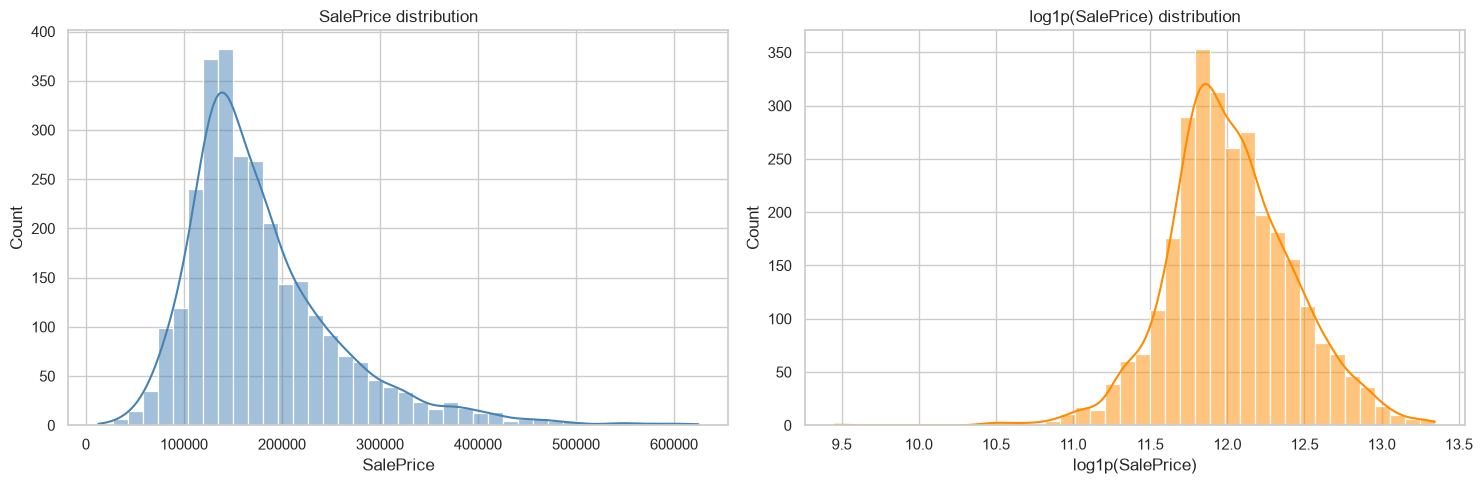
\includegraphics[width=\textwidth]{figures/saleprice_logprice_distributions.png}
  \caption{SalePrice and \(\log(1+\mathrm{SalePrice})\) distributions.}
  \label{fig:target-distributions}
\end{figure}

\section{Single-variable analysis}

Figure~\ref{fig:continuous-univariate} shows the continuous regressors against
sale price. Larger above-ground living area, newer construction or remodelling,
and larger basement and garage areas generally align with higher sale prices,
although dispersion rises for expensive homes. These are univariate descriptive
relationships and do not control for location, quality, or other property
characteristics.

\begin{figure}[H]
  \centering
  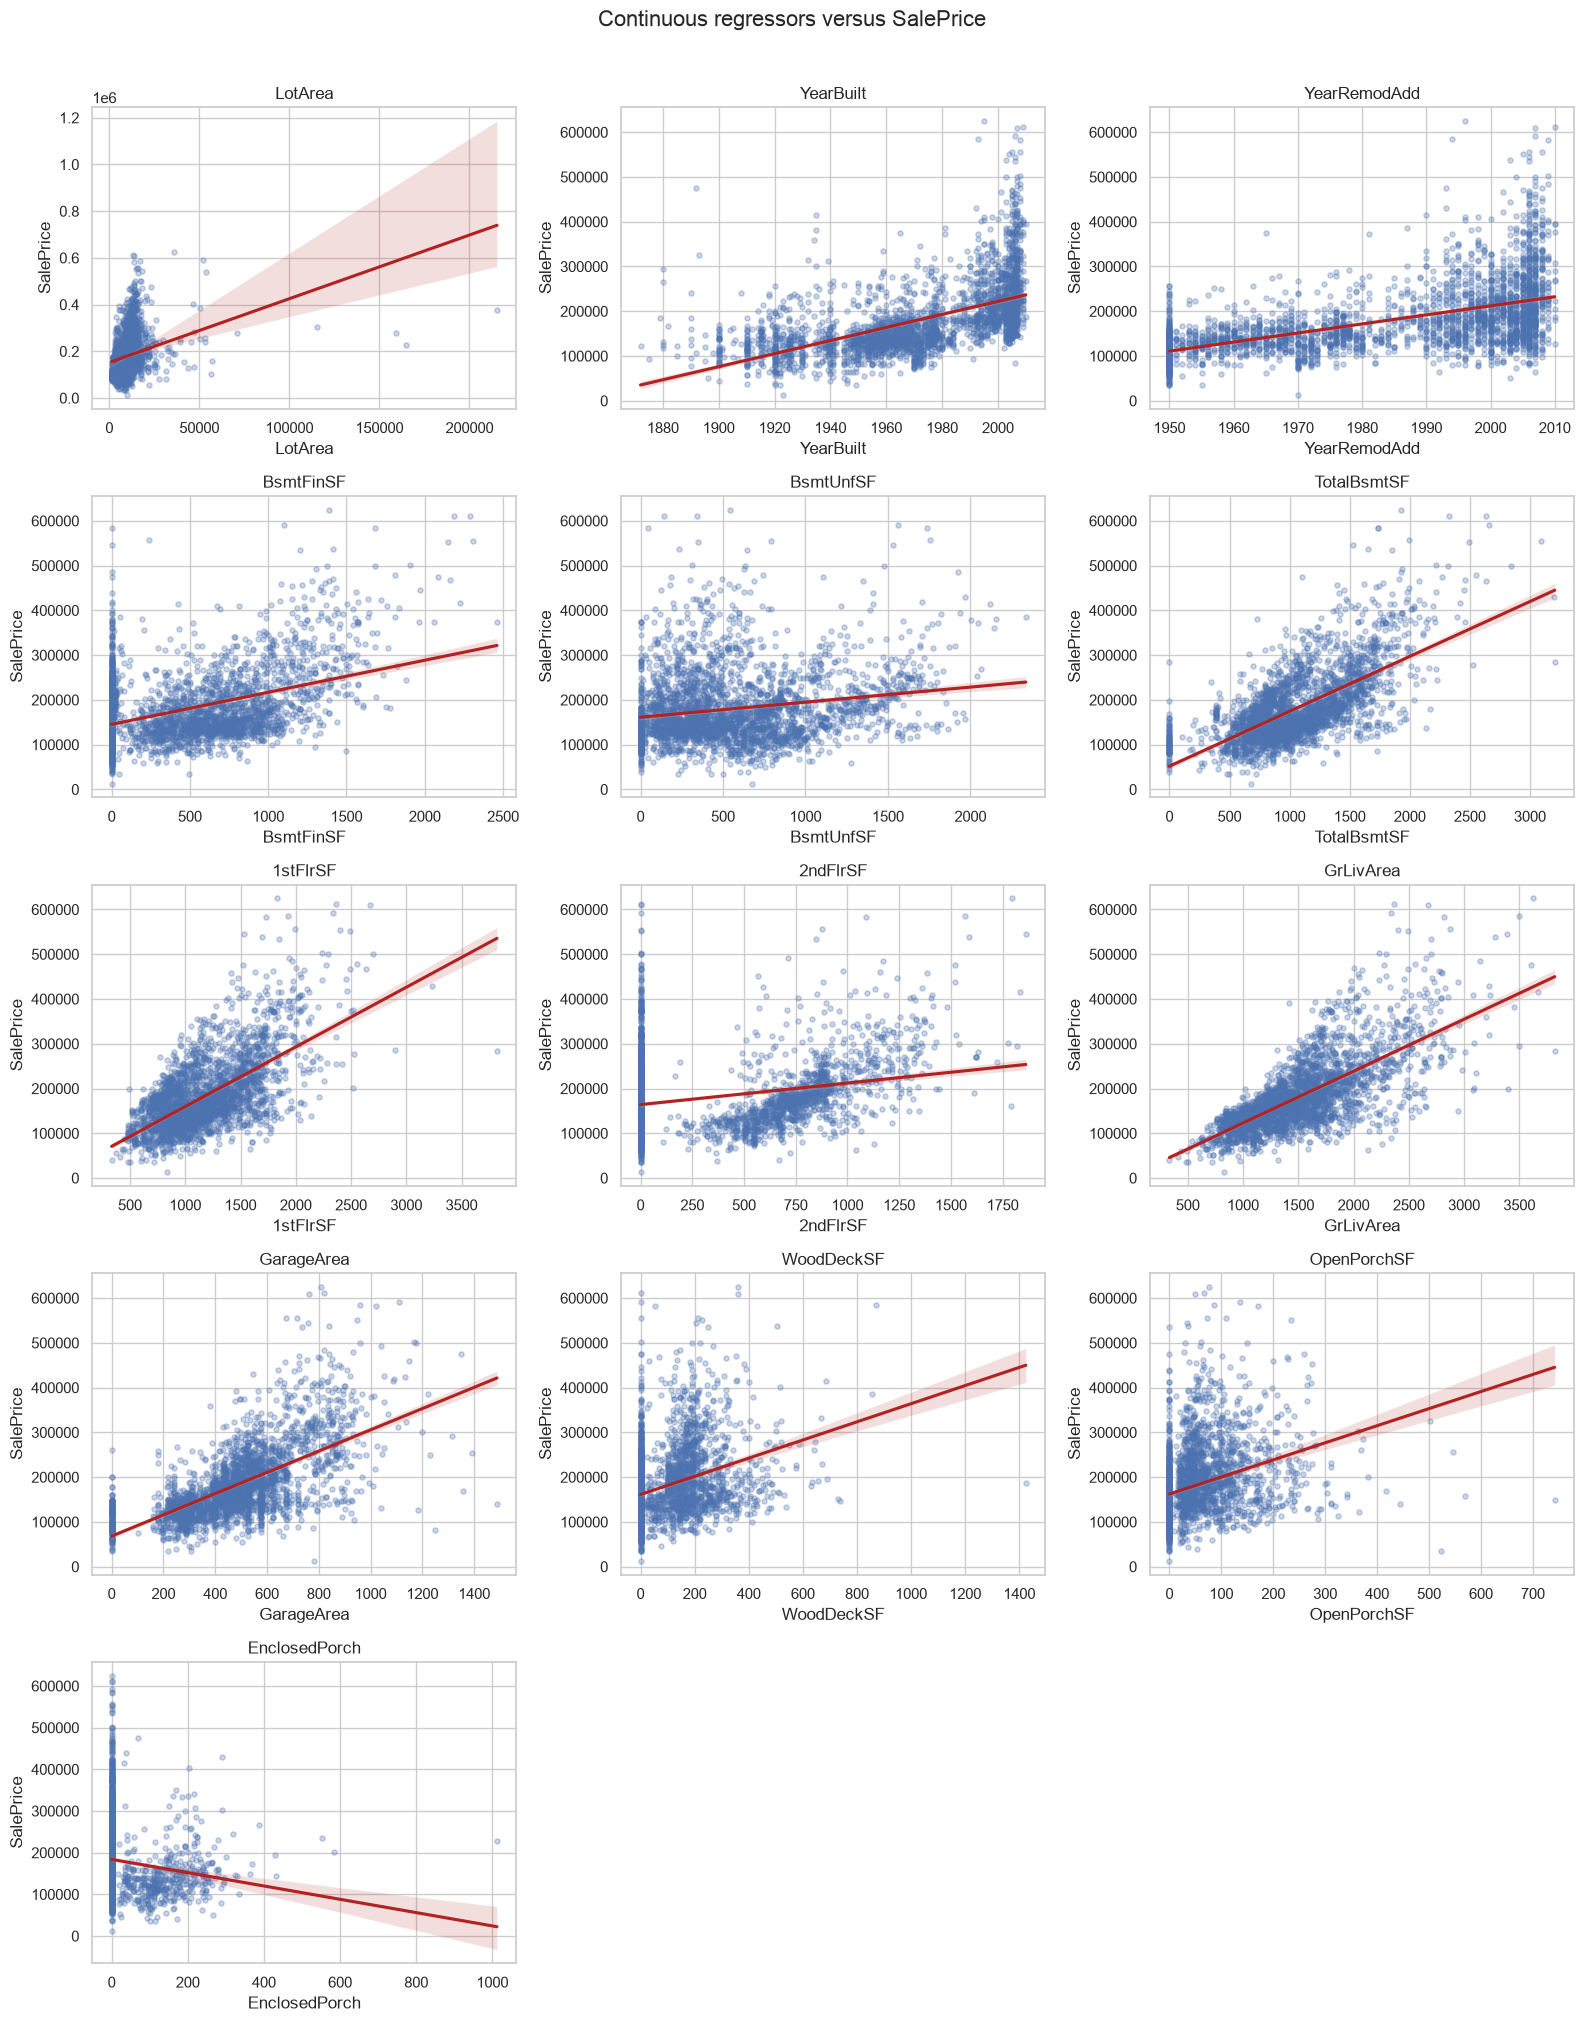
\includegraphics[width=0.92\textwidth,height=0.82\textheight,keepaspectratio]{figures/continuous_regressors_vs_saleprice.png}
  \caption{Continuous regressors versus SalePrice, with descriptive fitted lines.}
  \label{fig:continuous-univariate}
\end{figure}

Figure~\ref{fig:discrete-univariate} summarizes count and ordinal predictors.
The boxplots show how observed predictor values separate sale-price distributions.

\begin{figure}[H]
  \centering
  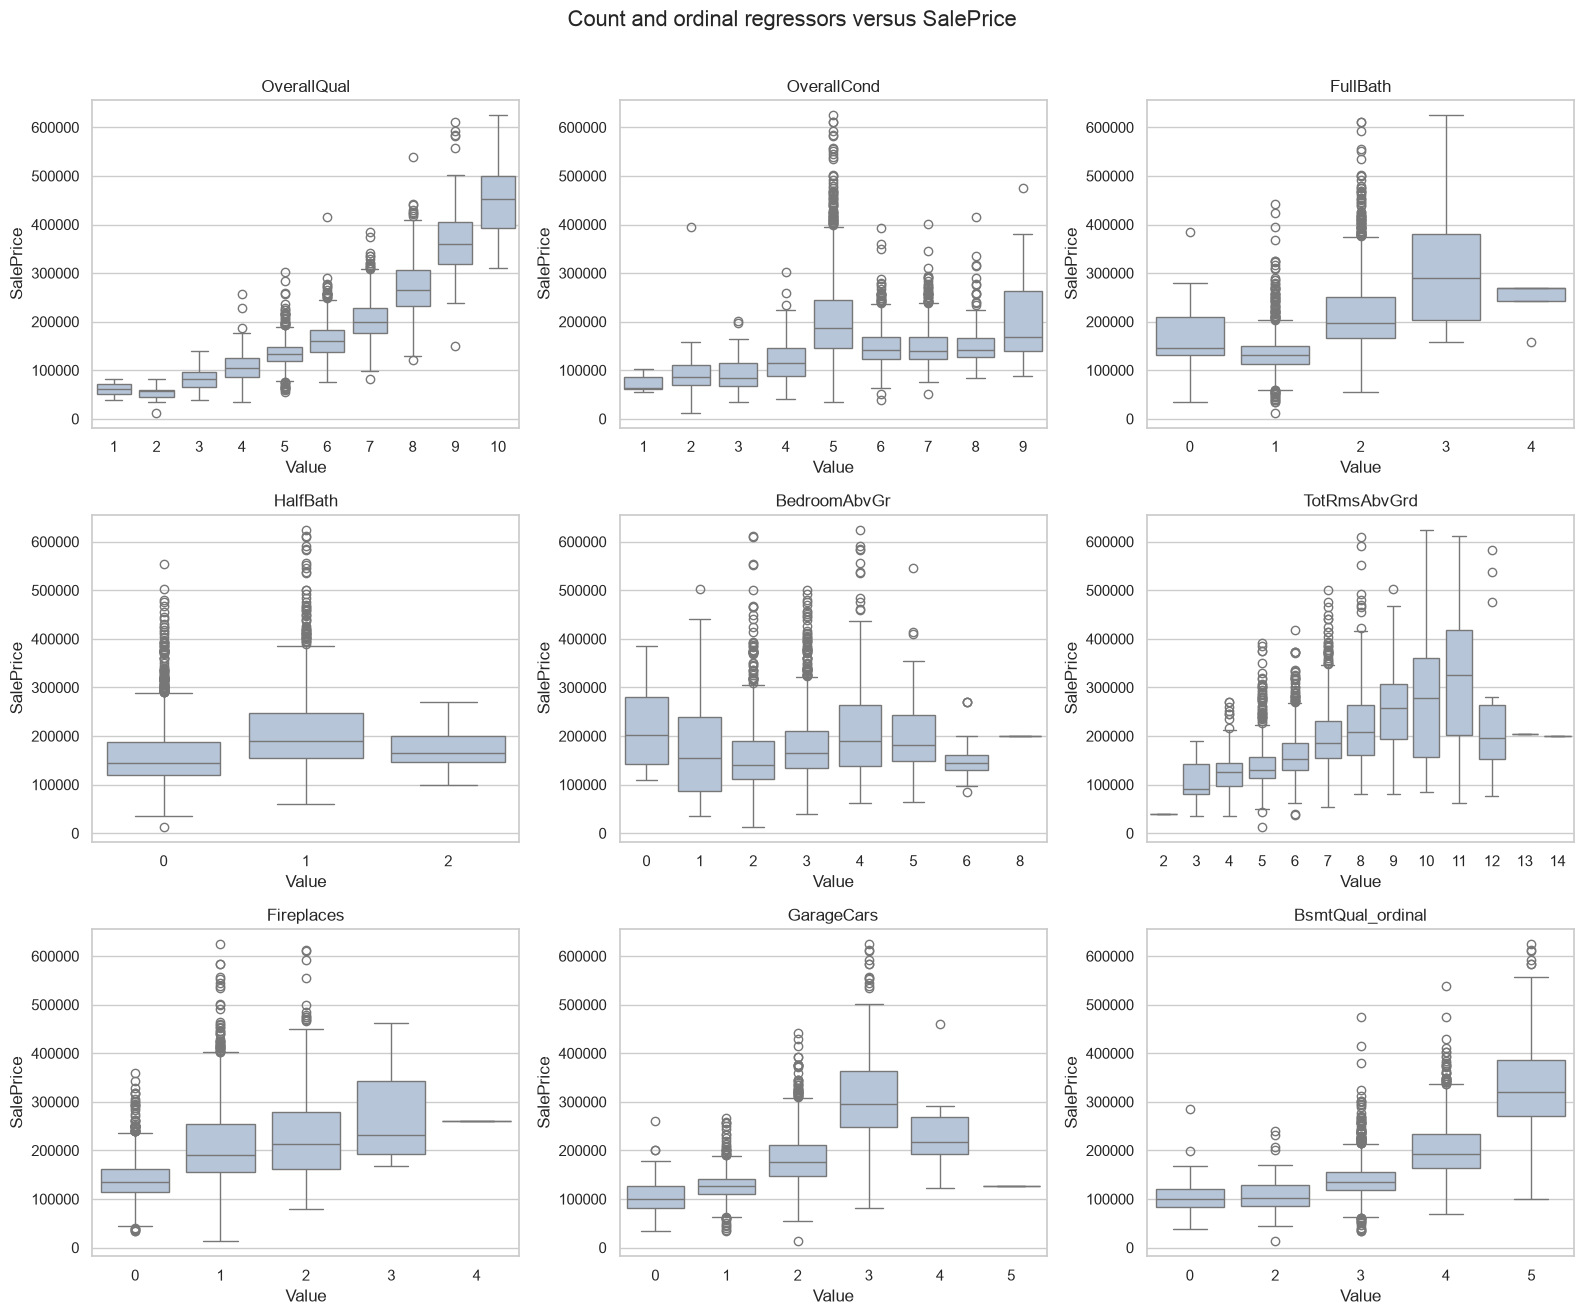
\includegraphics[width=0.92\textwidth,height=0.80\textheight,keepaspectratio]{figures/count_ordinal_regressors_vs_saleprice.png}
  \caption{Count and ordinal regressors versus SalePrice.}
  \label{fig:discrete-univariate}
\end{figure}

Location is also economically important. Figure~\ref{fig:neighborhood-univariate}
reports median sale price by neighborhood and labels each bar with its sample
size. The differing medians support retaining neighborhood indicators while the
sample-size labels caution against overinterpreting small groups.

\begin{figure}[H]
  \centering
  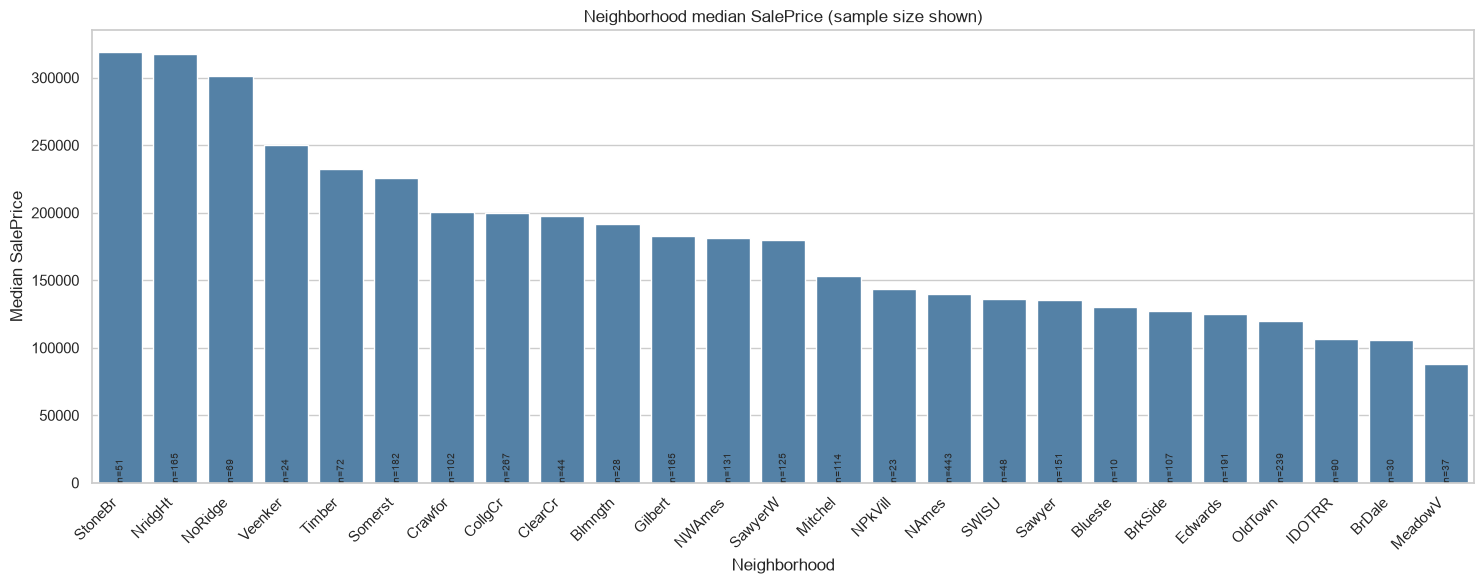
\includegraphics[width=0.94\textwidth]{figures/neighborhood_median_saleprice.png}
  \caption{Median SalePrice by neighborhood, with sample sizes.}
  \label{fig:neighborhood-univariate}
\end{figure}

\section{Correlation heatmap}

Figure~\ref{fig:continuous-correlation} displays Pearson correlations among the
13 continuous regressors used in the EDA notebook. Several physical-size
variables move together, particularly the basement-area measures. The resulting
correlation structure motivates caution when interpreting individual linear-model
coefficients in a specification that contains related size measures.

\begin{figure}[H]
  \centering
  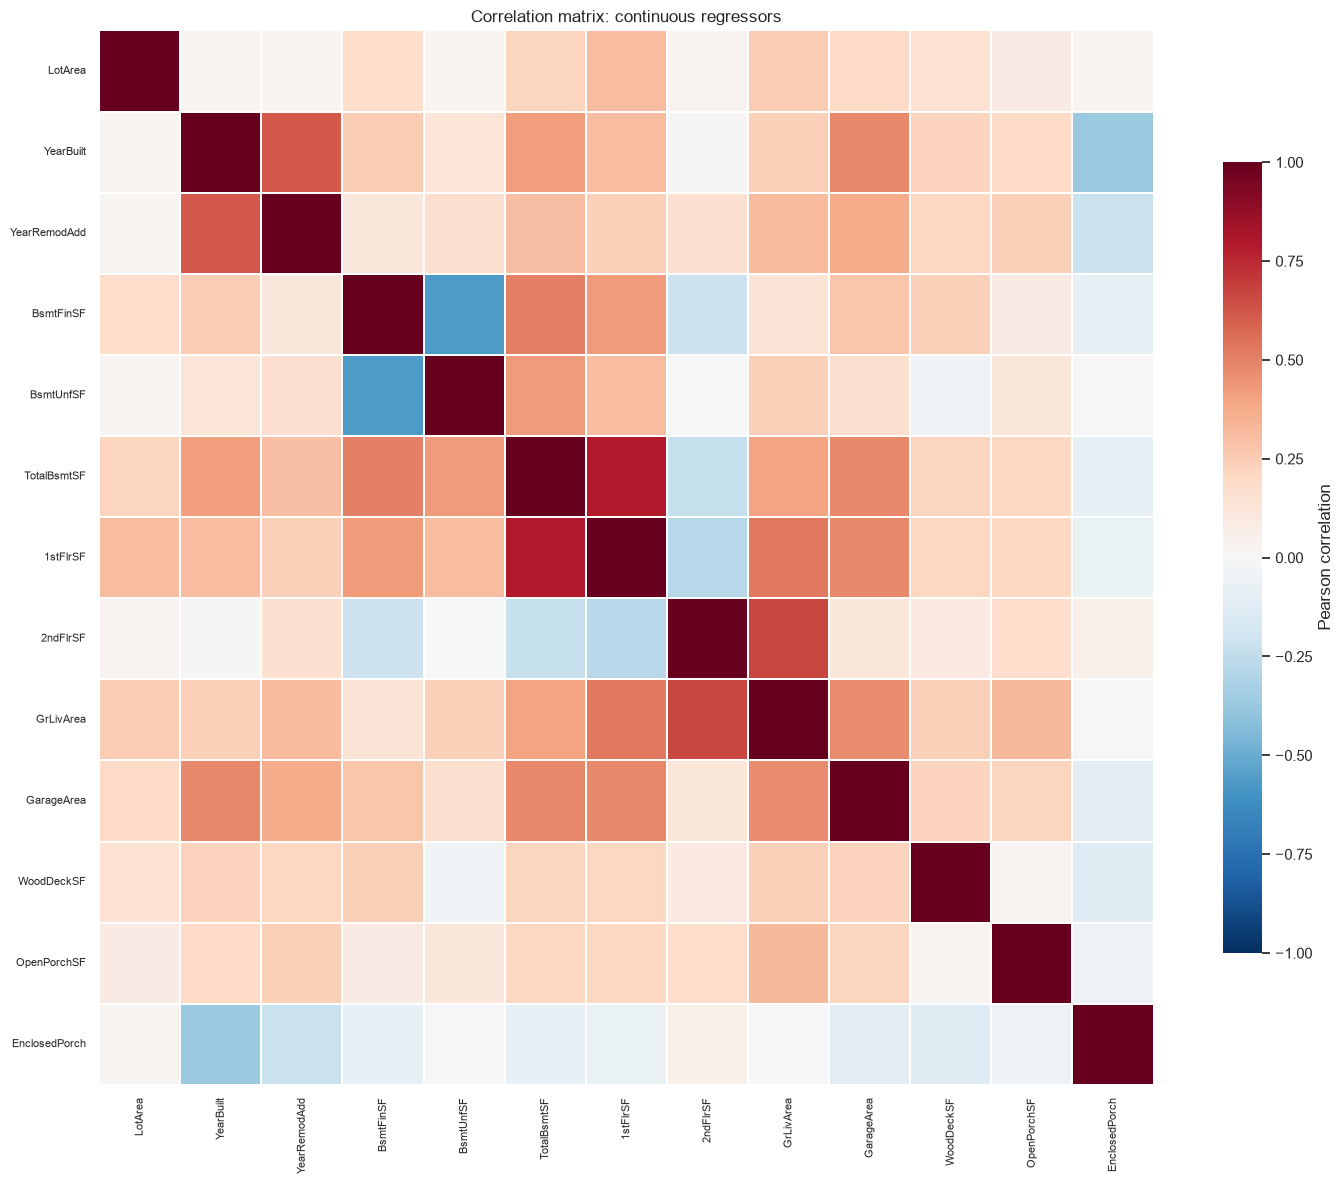
\includegraphics[width=0.92\textwidth]{figures/continuous_correlation_heatmap.png}
  \caption{Pearson-correlation heatmap for the 13 continuous regressors.}
  \label{fig:continuous-correlation}
\end{figure}

\end{document}
